\documentclass[twoside,11pt]{article}

\usepackage{graphicx}
\pagestyle{myheadings}

%  Copyright:
%     Copyright (C) 1998 Particle Physics and Astronomy
%     Research Council. All Rights Reserved.


%------------------------------------------------------------------------------
% Add any \newcommand or \newenvironment commands here
\newcommand{\about}{$\sim$}
\newcommand{\eg}{{\it e.g.}}
\newcommand{\ie}{{\it i.e.}}
\newcommand{\mic}{\mbox{\,${\mu}$m}}               % microns
\newcommand{\arcmin}{{$^\prime$}}
\newcommand{\degr}{\mbox{\,$^\circ$}}               % degrees sign
%------------------------------------------------------------------------------

% -----------------------------------------------------------------------------
% ? Document identification
\newcommand{\stardoccategory}  {MT User Note}
\newcommand{\stardocinitials}  {MTUN}
\newcommand{\stardocsource}    {MT/UN/\stardocnumber}
\newcommand{\stardocnumber}    {204.1}
\newcommand{\stardocauthors}   {G. Sandell \\ \jac}
\newcommand{\stardocdate}      {Dec 1998}
\newcommand{\stardoctitle}     {SCUBA map reduction:\\[2ex]
                                A short guide}
\newcommand{\stardocversion}   {MT/UN/204.1}
\newcommand{\stardocmanual}    {\ }
\newcommand{\stardocabstract}  {[Text of abstract]}
% ? End of document identification
 
% A new environment for quoting verbatim
% Environment for indenting and using a small font.
\newenvironment{myquote}{\begin{quote}\begin{small}}{\end{small}\end{quote}}
 
\newcommand{\text}[1]{{\small \texttt{#1}}}
 
% SCUBA reference
\newcommand{\scuba}{\htmladdnormallink{SCUBA}{http://www.jach.hawaii.edu/JCMT/}}

 
% Starlink Package names
\newcommand{\starlink}{\htmladdnormallink{Starlink}{http://star-www.rl.ac.uk/}}
 
% set up some common package names
\newcommand{\Kappa}{\xref{\textsc{Kappa}}{sun95}{}}
\newcommand{\Figaro}{\xref{\textsc{Figaro}}{sun86}{}}
\newcommand{\gaia}{\xref{\textsc{Gaia}}{sun214}{}}
\newcommand{\convert}{\xref{\textsc{Convert}}{sun55}{}}
\newcommand{\fluxes}{\xref{\textsc{Fluxes}}{sun213}{}}
\newcommand{\Iras}{\xref{\textsc{Iras90}}{sun163}{}}
\newcommand{\ndf}{\xref{NDF}{sun33}{}}
\newcommand{\agi}{\xref{AGI}{sun48}{}}
\newcommand{\surf}{\xref{\textsc{Surf}}{sun216}{}}
\newcommand{\Specdre}{\xref{\textsc{Specdre}}{sun140}{}}
\newcommand{\jcmtdr}{\xref{\textsc{JCMTdr}}{sun132}{}}
\newcommand{\nod}{\textsc{nod2}}
\newcommand{\ESP}{\xref{ESP}{sun180}{}}
\newcommand{\GKS}{\xref{GKS}{sun83}{}}

% Application tasks
\newcommand{\task}[1]{\textsf{#1}}
 
% ADAM parameters
\newcommand{\param}[1]{\texttt{#1}}
 
% SURF tasks
\newcommand{\rebin}{\xref{\task{rebin}}{sun216}{REBIN}}
\newcommand{\remdbm}{\xref{\task{remdbm}}{sun216}{REMDBM}}
\newcommand{\bolrebin}{\xref{\task{bolrebin}}{sun216}{BOLREBIN}}
\newcommand{\intrebin}{\xref{\task{intrebin}}{sun216}{INTREBIN}}
\newcommand{\calcsky}{\xref{\task{calcsky}}{sun216}{CALCSKY}}
\newcommand{\chgqual}{\xref{\task{change\_\-qua\-lity}}{sun216}{CHANGE_QUALITY}}
\newcommand{\chgflat}{\xref{\task{change\_flat}}{sun216}{CHANGE_FLAT}}
\newcommand{\chgpnt}{\xref{\task{change\_pointing}}{sun216}{CHANGE_POINTING}}
\newcommand{\chgdata}{\xref{\task{change\_data}}{sun216}{CHANGE_DATA}}
\newcommand{\desp}{\xref{\task{despike}}{sun216}{DESPIKE}}
%\newcommand{\desp2}{\xref{\task{despike2}}{sun216}{DESPIKE2}}
\newcommand{\dspbol}{\xref{\task{dspbol}}{sun216}{DSPBOL}}
\newcommand{\resw}{\xref{\task{reduce\_switch}}{sun216}{REDUCE_SWITCH}}
\newcommand{\flatf}{\xref{\task{flatfield}}{sun216}{FLATFIELD}}
\newcommand{\skydip}{\xref{\task{skydip}}{sun216}{SKYDIP}}

\newcommand{\scuphot}{\xref{\task{scuphot}}{sun216}{SCUPHOT}}
\newcommand{\scanrlb}{\xref{\task{scan\_rlb}}{sun216}{SCAN_RLB}}
\newcommand{\ext}{\xref{\task{extinction}}{sun216}{EXTINCTION}}
\newcommand{\scuquick}{\xref{\task{scuquick}}{sun216}{SCUQUICK}}
\newcommand{\scuhelp}{\xref{\task{scuhelp}}{sun216}{SCUHELP}}
\newcommand{\remsky}{\xref{\task{remsky}}{sun216}{REMSKY}}
\newcommand{\scuover}{\xref{\task{scuover}}{sun216}{SCUOVER}}
\newcommand{\extdata}{\xref{\task{extract\_data}}{sun216}{EXTRACT_DATA}}
\newcommand{\sculog}{\xref{\task{sculog}}{sun216}{SCULOG}}
\newcommand{\scuplot}{\xref{\task{scuplot}}{sun216}{SCUPLOT}}
\newcommand{\scucat}{\xref{\task{scucat}}{sun216}{SCUCAT}}
\newcommand{\photsum}{\xref{\task{photsum}}{sun216}{PHOTSUM}}
\newcommand{\mapsum}{\xref{\task{mapsum}}{sun216}{MAPSUM}}
\newcommand{\pointsum}{\xref{\task{pointsum}}{sun216}{POINTSUM}}
\newcommand{\qdraw}{\xref{\task{qdraw}}{sun216}{QDRAW}}
\newcommand{\sigclip}{\xref{\task{sigclip}}{sun216}{SIGCLIP}}
\newcommand{\restore}{\xref{\task{restore}}{sun216}{RESTORE}}
\newcommand{\sdip}{\xref{\task{sdip}}{sun216}{SDIP}}
\newcommand{\scuclip}{\xref{\task{scuclip}}{sun216}{SCUCLIP}}
\newcommand{\scupa}{\xref{\task{scupa}}{sun216}{SCUPA}}
\newcommand{\scunoise}{\xref{\task{scunoise}}{sun216}{SCUNOISE}}
\newcommand{\obssum}{\xref{\task{obssum}}{sun216}{OBSSUM}}
 
% Non surf tasks

% KAPPA 
\newcommand{\display}{\xref{\task{display}}{sun95}{DISPLAY}}
\newcommand{\aperadd}{\xref{\task{aperadd}}{sun95}{APERADD}}
\newcommand{\linplot}{\xref{\task{linplot}}{sun95}{LINPLOT}}
\newcommand{\mlinplot}{\xref{\task{mlinplot}}{sun95}{MLINPLOT}}
\newcommand{\drawsig}{\xref{\task{drawsig}}{sun95}{DRAWSIG}}
\newcommand{\centroid}{\xref{\task{centroid}}{sun95}{CENTROID}}
\newcommand{\hislist}{\xref{\task{hislist}}{sun95}{HISLIST}}
\newcommand{\globals}{\xref{\task{globals}}{sun95}{GLOBALS}}
\newcommand{\setaxis}{\xref{\task{setaxis}}{sun95}{SETAXIS}}
\newcommand{\kstest}{\xref{\task{kstest}}{sun95}{KSTEST}}
\newcommand{\stats}{\xref{\task{stats}}{sun95}{STATS}}
\newcommand{\thresh}{\xref{\task{thresh}}{sun95}{THRESH}}
\newcommand{\setbb}{\xref{\task{setbb}}{sun95}{SETBB}}

\newcommand{\fitslist}{\xref{\task{fitslist}}{sun95}{FITSLIST}}
\newcommand{\fitsedit}{\xref{\task{fitsedit}}{sun95}{FITSEDIT}}

\newcommand{\setvar}{\xref{\task{setvar}}{sun95}{SETVAR}}
\newcommand{\ndfcopy}{\xref{\task{ndfcopy}}{sun95}{NDFCOPY}}
\newcommand{\gdset}{\xref{\task{gdset}}{sun95}{GDSET}}
\newcommand{\idset}{\xref{\task{idset}}{sun95}{IDSET}}
\newcommand{\ovset}{\xref{\task{ovset}}{sun95}{OVSET}}
\newcommand{\gdnames}{\xref{\task{gdnames}}{sun95}{GDNAMES}}
\newcommand{\gdclear}{\xref{\task{gdclear}}{sun95}{GDCLEAR}}
\newcommand{\cursor}{\xref{\task{cursor}}{sun95}{CURSOR}}
\newcommand{\flip}{\xref{\task{flip}}{sun95}{FLIP}}
\newcommand{\cadd}{\xref{\task{cadd}}{sun95}{CADD}}

\newcommand{\cdiv}{\xref{\task{cdiv}}{sun95}{CDIV}}
\newcommand{\Div}{\xref{\task{div}}{sun95}{DIV}}
\newcommand{\cmult}{\xref{\task{cmult}}{sun95}{CMULT}}
\newcommand{\mult}{\xref{\task{mult}}{sun95}{MULT}}
\newcommand{\add}{\xref{\task{add}}{sun95}{ADD}}
\newcommand{\sub}{\xref{\task{sub}}{sun95}{SUB}}
\newcommand{\csub}{\xref{\task{csub}}{sun95}{CSUB}}
\newcommand{\psf}{\xref{\task{psf}}{sun95}{PSF}}

\newcommand{\glitch}{\xref{\task{glitch}}{sun95}{GLITCH}}
\newcommand{\setunits}{\xref{\task{setunits}}{sun95}{SETUNITS}}
\newcommand{\fitstext}{\xref{\task{fitstext}}{sun95}{FITSTEXT}}
\newcommand{\fitsmod}{\xref{\task{fitsmod}}{sun95}{FITSMOD}}
\newcommand{\fitshead}{\xref{\task{fitshead}}{sun95}{FITSHEAD}}
\newcommand{\lutbgyrw}{\xref{\task{lutbgyrw}}{sun95}{LUTBGYRW}}
\newcommand{\contour}{\xref{\task{contour}}{sun95}{CONTOUR}}
\newcommand{\contover}{\xref{\task{contover}}{sun95}{CONTOVER}}

\newcommand{\turbocont}{\xref{\task{turbocont}}{sun95}{TURBOCONT}}
\newcommand{\mosaic}{\xref{\task{mosaic}}{sun95}{MOSAIC}}
\newcommand{\pixdupe}{\xref{\task{pixdupe}}{sun95}{PIXDUPE}}
\newcommand{\rotate}{\xref{\task{rotate}}{sun95}{ROTATE}}
\newcommand{\setbound}{\xref{\task{setbound}}{sun95}{SETBOUND}}
\newcommand{\slide}{\xref{\task{slide}}{sun95}{SLIDE}}
\newcommand{\gausmooth}{\xref{\task{gausmooth}}{sun95}{GAUSMOOTH}}
\newcommand{\median}{\xref{\task{median}}{sun95}{MEDIAN}}

\newcommand{\memd}{\xref{\task{mem2d}}{sun95}{MEM2D}}
\newcommand{\axlabel}{\xref{\task{axlabel}}{sun95}{AXLABEL}}
\newcommand{\axunits}{\xref{\task{axunits}}{sun95}{AXUNITS}}
\newcommand{\setlabel}{\xref{\task{setlabel}}{sun95}{SETLABEL}}
\newcommand{\settitle}{\xref{\task{settitle}}{sun95}{SETTITLE}}
\newcommand{\histogram}{\xref{\task{histogram}}{sun95}{HISTOGRAM}}
\newcommand{\normalize}{\xref{\task{normalize}}{sun95}{NORMALIZE}}

% Convert
\newcommand{\ndffits}{\xref{\task{ndf2fits}}{sun55}{NDF2FITS}}
\newcommand{\ndfascii}{\xref{\task{ndf2ascii}}{sun55}{NDF2ASCII}}

% FIGARO
\newcommand{\wdfits}{\xref{\task{wdfits}}{sun86}{WDFITS}}
\newcommand{\istat}{\xref{\task{istat}}{sun86}{ISTAT}}
\newcommand{\delobj}{\xref{\task{delobj}}{sun86}{DELOBJ}}
\newcommand{\copobj}{\xref{\task{copobj}}{sun86}{COPOBJ}}
\newcommand{\image}{\xref{\task{image}}{sun86}{IMAGE}}
\newcommand{\bclean}{\xref{\task{bclean}}{sun86}{BCLEAN}}
\newcommand{\ystract}{\xref{\task{ystract}}{sun86}{YSTRACT}}

% IRAS90
\newcommand{\skypos}{\xref{\task{skypos}}{sun163}{SKYPOS}}
\newcommand{\skygrid}{\xref{\task{skygrid}}{sun163}{SKYGRID}}
\newcommand{\skyphot}{\xref{\task{skyphot}}{sun163}{SKYPHOT}}


% Misc
\newcommand{\hdstrace}{\xref{\task{hdstrace}}{sun102}{}}
\newcommand{\psmerge}{\xref{\task{psmerge}}{sun164}{}}
\newcommand{\fitgauss}{\xref{\task{fitgauss}}{sun140}{FITGAUSS}}
\newcommand{\gaufit}{\xref{\task{gaufit}}{sun180}{GAUFIT}}

% JAC

\newcommand{\jac}{\htmladdnormallink{Joint Astronomy Centre}{http://www.jach.hawaii.edu},
 Hilo, Hawaii}

% +
%  Name:
%     sc.tex
%
%  Purpose:
%     Template for Starlink Cookbook (SC) documents.
%     Refer to SUN/199
%
%  Authors:
%     AJC: A.J.Chipperfield (Starlink, RAL)
%     BLY: M.J.Bly (Starlink, RAL)
%     PWD: Peter W. Draper (Starlink, Durham University)
%
%  History:
%     16-JUN-1997 (BLY):
%        Original, based on SUN/SG templates.
%     13-AUG-1998 (PWD):
%        Converted for use with LaTeX2HTML version 98.2 and
%        Star2HTML version 1.3.
%     {Add further history here}
%
% -

\newcommand{\stardocname}{\stardocinitials /\stardocnumber}
\markboth{\stardocname}{\stardocname}
\setlength{\textwidth}{160mm}
\setlength{\textheight}{230mm}
\setlength{\topmargin}{-2mm}
\setlength{\oddsidemargin}{0mm}
\setlength{\evensidemargin}{0mm}
\setlength{\parindent}{0mm}
\setlength{\parskip}{\medskipamount}
\setlength{\unitlength}{1mm}

% -----------------------------------------------------------------------------
%  Hypertext definitions.
%  ======================
%  These are used by the LaTeX2HTML translator in conjunction with star2html.

%  Comment.sty: version 2.0, 19 June 1992
%  Selectively in/exclude pieces of text.
%
%  Author
%    Victor Eijkhout                                      <eijkhout@cs.utk.edu>
%    Department of Computer Science
%    University Tennessee at Knoxville
%    104 Ayres Hall
%    Knoxville, TN 37996
%    USA

%  Do not remove the %begin{latexonly} and %end{latexonly} lines (used by 
%  LaTeX2HTML to signify text it shouldn't process).
%begin{latexonly}
\makeatletter
\def\makeinnocent#1{\catcode`#1=12 }
\def\csarg#1#2{\expandafter#1\csname#2\endcsname}

\def\ThrowAwayComment#1{\begingroup
    \def\CurrentComment{#1}%
    \let\do\makeinnocent \dospecials
    \makeinnocent\^^L% and whatever other special cases
    \endlinechar`\^^M \catcode`\^^M=12 \xComment}
{\catcode`\^^M=12 \endlinechar=-1 %
 \gdef\xComment#1^^M{\def\test{#1}
      \csarg\ifx{PlainEnd\CurrentComment Test}\test
          \let\html@next\endgroup
      \else \csarg\ifx{LaLaEnd\CurrentComment Test}\test
            \edef\html@next{\endgroup\noexpand\end{\CurrentComment}}
      \else \let\html@next\xComment
      \fi \fi \html@next}
}
\makeatother

\def\includecomment
 #1{\expandafter\def\csname#1\endcsname{}%
    \expandafter\def\csname end#1\endcsname{}}
\def\excludecomment
 #1{\expandafter\def\csname#1\endcsname{\ThrowAwayComment{#1}}%
    {\escapechar=-1\relax
     \csarg\xdef{PlainEnd#1Test}{\string\\end#1}%
     \csarg\xdef{LaLaEnd#1Test}{\string\\end\string\{#1\string\}}%
    }}

%  Define environments that ignore their contents.
\excludecomment{comment}
\excludecomment{rawhtml}
\excludecomment{htmlonly}

%  Hypertext commands etc. This is a condensed version of the html.sty
%  file supplied with LaTeX2HTML by: Nikos Drakos <nikos@cbl.leeds.ac.uk> &
%  Jelle van Zeijl <jvzeijl@isou17.estec.esa.nl>. The LaTeX2HTML documentation
%  should be consulted about all commands (and the environments defined above)
%  except \xref and \xlabel which are Starlink specific.

\newcommand{\htmladdnormallinkfoot}[2]{#1\footnote{#2}}
\newcommand{\htmladdnormallink}[2]{#1}
\newcommand{\htmladdimg}[1]{}
\newcommand{\hyperref}[4]{#2\ref{#4}#3}
\newcommand{\htmlref}[2]{#1}
\newcommand{\htmlimage}[1]{}
\newcommand{\htmladdtonavigation}[1]{}

\newenvironment{latexonly}{}{}
\newcommand{\latex}[1]{#1}
\newcommand{\html}[1]{}
\newcommand{\latexhtml}[2]{#1}
\newcommand{\HTMLcode}[2][]{}

%  Starlink cross-references and labels.
\newcommand{\xref}[3]{#1}
\newcommand{\xlabel}[1]{}

%  LaTeX2HTML symbol.
\newcommand{\latextohtml}{\LaTeX2\texttt{HTML}}

%  Define command to re-centre underscore for Latex and leave as normal
%  for HTML (severe problems with \_ in tabbing environments and \_\_
%  generally otherwise).
\renewcommand{\_}{\texttt{\symbol{95}}}

% -----------------------------------------------------------------------------
%  Debugging.
%  =========
%  Remove % on the following to debug links in the HTML version using Latex.

% \newcommand{\hotlink}[2]{\fbox{\begin{tabular}[t]{@{}c@{}}#1\\\hline{\footnotesize #2}\end{tabular}}}
% \renewcommand{\htmladdnormallinkfoot}[2]{\hotlink{#1}{#2}}
% \renewcommand{\htmladdnormallink}[2]{\hotlink{#1}{#2}}
% \renewcommand{\hyperref}[4]{\hotlink{#1}{\S\ref{#4}}}
% \renewcommand{\htmlref}[2]{\hotlink{#1}{\S\ref{#2}}}
% \renewcommand{\xref}[3]{\hotlink{#1}{#2 -- #3}}
%end{latexonly}
% -----------------------------------------------------------------------------
% ? Document specific \newcommand or \newenvironment commands.
% ? End of document specific commands
% -----------------------------------------------------------------------------
%  Title Page.
%  ===========
\renewcommand{\thepage}{\roman{page}}
\begin{document}
\thispagestyle{empty}

%  Latex document header.
%  ======================
\begin{latexonly}
   CCLRC / {\textsc Rutherford Appleton Laboratory} \hfill {\textbf \stardocname}\\
   {\large Particle Physics \& Astronomy Research Council}\\
   {\large Starlink Project\\}
   {\large \stardoccategory\ \stardocnumber}
   \begin{flushright}
   \stardocauthors\\
   \stardocdate
   \end{flushright}
   \vspace{-4mm}
   \rule{\textwidth}{0.5mm}
   \vspace{5mm}
   \begin{center}
   {\Huge\textbf  \stardoctitle \\ [2.5ex]}
   {\LARGE\textbf \stardocversion \\ [4ex]}
   {\Huge\textbf  \stardocmanual}
   \end{center}
%   \vspace{5mm}

% ? Add picture here if required for the LaTeX version.
%   e.g. \includegraphics[scale=0.3]{filename.ps}
\begin{center}

\includegraphics[width=2.0in]{sc11_logo.eps}
\end{center}
% ? End of picture

% ? Heading for abstract if used.
%   \vspace{10mm}
%   \begin{center}
%      {\Large\textbf Abstract}
%   \end{center}
% ? End of heading for abstract.
\end{latexonly}

%  HTML documentation header.
%  ==========================
\begin{htmlonly}
   \xlabel{}
   \begin{rawhtml} <H1 ALIGN=CENTER> \end{rawhtml}
      \stardoctitle\\
      \stardocversion\\
      \stardocmanual
   \begin{rawhtml} </H1> <HR> \end{rawhtml}

% ? Add picture here if required for the hypertext version.
%   e.g. \includegraphics[scale=0.7]{filename.ps}

\includegraphics[width=2.0in]{sc11_logo.eps}
% ? End of picture

   \begin{rawhtml} <P> <I> \end{rawhtml}
   \stardoccategory\ \stardocnumber \\
   \stardocauthors \\
   \stardocdate
   \begin{rawhtml} </I> </P> <H3> \end{rawhtml}
      \htmladdnormallink{CCLRC}{http://www.cclrc.ac.uk} /
      \htmladdnormallink{Rutherford Appleton Laboratory}
                        {http://www.cclrc.ac.uk/ral} \\
      \htmladdnormallink{Particle Physics \& Astronomy Research Council}
                        {http://www.pparc.ac.uk} \\
   \begin{rawhtml} </H3> <H2> \end{rawhtml}
      \htmladdnormallink{Starlink Project}{http://star-www.rl.ac.uk/}
   \begin{rawhtml} </H2> \end{rawhtml}
   \htmladdnormallink{\htmladdimg{source.gif} Retrieve hardcopy}
      {http://star-www.rl.ac.uk/cgi-bin/hcserver?\stardocsource}\\

%  HTML document table of contents. 
%  ================================
%  Add table of contents header and a navigation button to return to this 
%  point in the document (this should always go before the abstract \section). 
  \label{stardoccontents}
  \begin{rawhtml} 
    <HR>
    <H2>Contents</H2>
  \end{rawhtml}
  \htmladdtonavigation{\htmlref{\htmladdimg{contents_motif.gif}}
        {stardoccontents}}

% ? New section for abstract if used.
%  \section{\xlabel{abstract}Abstract}
% ? End of new section for abstract
\end{htmlonly}

% -----------------------------------------------------------------------------
% ? Document Abstract. (if used)
%  ==================
%\stardocabstract
% ? End of document abstract
% -----------------------------------------------------------------------------
% ? Latex document Table of Contents (if used).
%  ===========================================
  \newpage
  \begin{latexonly}
    \setlength{\parskip}{0mm}
    \tableofcontents
    \setlength{\parskip}{\medskipamount}
    \markboth{\stardocname}{\stardocname}
  \end{latexonly}
% ? End of Latex document table of contents
% -----------------------------------------------------------------------------
\cleardoublepage
\renewcommand{\thepage}{\arabic{page}}
\setcounter{page}{1}


\section{\xlabel{introduction}Introduction}

This is the short guide on how to quickly reduce, and analyze maps obtained
with \scuba\ using the off line SCUBA reduction package \surf\ \cite{surf} and
the \starlink\ versions of \Kappa \cite{kappa}, \Figaro \cite{figaro},
\gaia \cite{gaia}, and \convert \cite{convert} .  

This cookbook makes no attempts to explain why and how, for that there is a comprehensive Starlink User Note
(\xref{\textbf{SUN/216}}{sun216}{}) written by T. Jenness and J. Lightfoot,
which properly documents all the software tasks in \surf, which should be
consulted for those who need to know details of a task, or how the task
really works. 




\section{\xlabel{how_to_get_started}How to get started}

Log in on a unix workstation either in Hilo or at JCMT and create a 
directory where you want to store your reduced data. Next type

\begin{myquote}
\begin{verbatim}
% surf
% kappa
% figaro
% convert
\end{verbatim}
\end{myquote}

This starts up the scuba software and the main \starlink\ packages
needed for the data reduction.

The next thing you will need to do is to find the data and create
logs of your observing run, so that you know what scan numbers to reduce.


\subsection{\xlabel{how_to_find}How to find and access SCUBA data?}

All SCUBA data are stored on disk at
\htmladdnormallink{JAC}{http://www.jach.hawaii.edu/} and also for a
shorter period at JCMT. The data are initially stored on the summit
VAX, and copied to a unix disk (mounted as \texttt{/jcmtarchive}) after
each observation is completed.  Each night a new subdirectory is
created using the convention of year month and UT date, i.e. 19980215,
would contain data for the night between the 14th and 15th of February
1998. As of now data obtained on  for example the evening shift of Feb
15 are stored on the Vax in
\begin{myquote}
\begin{verbatim}
scuba_disk:[scuba.observe.19980215]
\end{verbatim}  
\end{myquote}

and copied to Hilo the following day, where they reside in a UNIX
directory:
\begin{myquote}
\begin{verbatim}
/scuba/m98a/19980215
\end{verbatim}
\end{myquote}
The directory structure in Hilo is a little different to that on the summit.
Data are stored in semester directories containing the UT date directories.
These UT date directories then only contain the demodulated data with the
RO files in an ro directory (in the semester directory) which contains
directories for each UT date).

On the vax raw maps, i.e. demodulated data, are stored in a subdirectory [.dem],
while the on-line reduced maps are stored in another subdirectory
[.ro], where \texttt{dem} stands for demodulated and \texttt{ro} for
reduced observations. 

For the data reduction and to get a listing of the data you want to
reduce you should now set up three environment variables, i.e. type the
following if you are logged on a Hilo workstation and if the data have
already been copied to Hilo:

\begin{myquote}
\begin{verbatim}
% setenv DATADIR /scuba/m9xa/199xmmdd/
% setenv SCUBA_PREFIX 199xmmdd
% setenv HDS_SCRATCH /tmp
\end{verbatim} 
\end{myquote}

Here x stands for the year, mm is the month (as a numeral), dd is the UT
date for the night you want to reduce and `a' is the semester letter
(\textit{a} or \textit{b}), i.e. 19980401 would be the night 
between March 31st and April 1st in 1998 and is in semester m98a.

If the data are still not copied to Hilo you can access the data from by
setting your DATADIR as

\begin{myquote} 
\begin{verbatim}
% setenv DATADIR /net/ieie/jcmtarchive/199xmmdd
\end{verbatim} 
\end{myquote}


In this case there no need to specify \texttt{dem} and you will
automatically get the raw data. If you are logged in at the summit you
should drop the first part of the specifier, i.e. \texttt{/net/ieie}.

You are now ready for creating a log of all maps obtained during the nigth
by typing:

\begin{myquote}
\begin{verbatim}
% mapsum -all -reduced > maps.log
\end{verbatim} 
\end{myquote}

Here I am piping the summary into a textfile, which called
\texttt{maplog.sum}.  You can choose any name you want. This is a simple
ASCII-file, which you can edit and print. I normally edit the file to inlude
my reduction notes and I'll print work copies in landscape mode by using the
unix command \texttt{enscript}, i.e. \texttt{enscript -r -d upstairs
maps.log}. The same we can make summaries of photometry (\texttt{photsum})
which may aid us to track extinction and calibration and \texttt{pointsum},
which gives us a pointing log, which we will need if we want to do astrometry
on our images.

\section{\xlabel{Jiggle_maps}Jiggle maps}
\subsection{\xlabel{The_first_steps}The first steps, \scuquick\ and extintion correction}
The basic SCUBA jiggle map reduction consists of 4 steps, each of which
is done with a separate task: \resw, \flatf, \ext\ and \rebin. These
can all be accessed through a script called \scuquick, which is written
to automate the whole reduction process. For a complete reduction, you
will also need some or all of the following tasks: \chgflat, \chgpnt,
\chgqual, \texttt{despike},  \remsky, \scuclip, and \scuover. For interactive
despiking you will also need to script \dspbol and for conventional
scan map data the tasks \restore\ and \desp2.

The script \scuquick\ is unix like , in the sense that one can invoke
qualifiers to specify input values and options. Standard usage of
\scuquick\ will be clear from the exaples below, but if you need more
information you can use the help option (\texttt{scuquick -h}) to get a
complete listing.  What you need in order to reduce your map is the
scan number of the map and the optical depth for the filter that you
want to reduce. For standard 850/450$\mu$m--maps you can get the
optical depth at 850 from skydips (which are given in the map summary),
but if you want to be careful you should also reduce it by \skydip,
i.e. type \texttt{skydip} and take defaults. Most of the time I derive
the 850$\mu$ opacity from $\tau_{CSO}$ using the formula


\begin{equation}
\tau_{850} = 4.3 \times (\tau_{CSO} - 0.028)
\end{equation}

which has a different zero point from the relation used by the SCUBA
team.  I have never found 450$\mu$m skydips to be reliable, and I
therefore derive the 450$\mu$m optical depth from $\tau_{CSO}$ by using

\begin{equation}
\tau_{450} = k \times (\tau_{CSO} - 0.01) + 0.02
\end{equation}

where k is a constant, which is not accurately known. I have tried different  values for k, and finally adopted 23, which works reasonably well. If $\tau_{CSO}$ is not working I derive it from the 850$\mu$m skydip
and then plug it in to the above formula to get $\tau_{450}$.

We now try our first map (scan 86), which is a single observation (3
integrations) of IRC+10216, one of our secondary calibrators, obtained
on December 8 1997. We set the environment variables DATADIR and
SCUBA\_PREFIX and run \scuquick\ for the long wavelength array (I find
it easier to do one array at a time) with an optical depth of 0.09 and
immediately display it to identify bad bolometers.  I do this with
the \Kappa\ command \display \footnote{\display\ is controlled by a
parameter \texttt{cosys}, which displays pixels if set to world, integrations or
arcsec, when set to data, e.g. \texttt{display axes clear cosys=data}},
and if \display\ is used for the first time, I have to set a color
table (I normally use \texttt{lutbgyrw}).

\begin{myquote}
\begin{verbatim}
% setenv DATADIR /scuba/observe/19971208/dem
% setenv SCUBA_PREFIX 19971208
% scuquick -tau=0.185 -sub=lon in 86 out=i86
Processing 19971208_dem_0086
SURF: Opening 19971208_dem_0086 in /scuba/observe/19971208/dem
SURF: run 86 was a MAP observation of object IRC+10216
SURF: file contains data for 2 switch(es) in 4 exposure(s) in
 3 integration(s) in 1 measurement(s)
SURF: run 86 was a MAP observation of IRC+10216
SURF: applying flatfield from lwswphot.dat
 
Processing the lon sub instrument
 
SURF: run 86 was a MAP observation with JIGGLE sampling of object IRC+10216
SURF: file contains data for 4 exposure(s) in 3 integration(s) in 1
measurement(s)
SURF: observation started at sidereal time 9 41 05 and ended at 9 50 09
SURF: file contains data for the following sub-instrument(s)
 - SHORT with filter 450
 - LONG with filter 850
Extinction corrected data has been written to file i86_lon_ext.sdf
% lutbgyrw
% display axes clear fill
IN - NDF to be displayed /@i86_lon_ext/ >
DEVICE - Name of display device /@xwindows/ > 
MODE - Method to define the scaling limits /'fa'/ > 
Data will be scaled from -0.0015181509079412 to 0.016302395612001.
\end{verbatim}
\end{myquote}

\subsection{\xlabel{Blanking_and_remsky}Blanking bad bolometers and sky noise removal}

\begin{figure}
\begin{center}
%%\epsfig{width=6.0in,file=sho_fig1.eps}
\includegraphics[width=5.5in]{sho_fig1.eps}
\caption{The extinction
corrected image of IRC+10216 without despiking and sky removal. In this image the bolometers are on the x-axis and the y-axis is time. Sky noise variations,
which occur at the same time for all pixels are easily seen, e.g.\ at the beginning of integration 2}
\label{fig:raw}
\end{center}
\end{figure}


\subsubsection{\xlabel{Blanking}How to identify and blank noisy bolometers.}

From the plot shown in Fig. \ \ref{fig:raw} we can see that the map suffers
from some sky noise, e.g. visible as the dark striping at the beginning of
integration 2.  The central bolometer, 19 (h7) shows a clear signal, and we do
not see any really bad (noisy) bolometers. Even so, we first need to blank out
bad bolometers. There are several ways to identify bad bolometers. The easiest
way, although it may not pick up all noisy bolometers for your particular map,
is to run \scunoise, which is a GUI that allows you to plot and identify all
noisy bolometers using noise measurements done during the run.  If we do this
for the night of 19971208 we find a total of 9 noise measurements and we can
see that some bolometers come and go, but 23 is always noisy.  From the most
nearby noise measurement, \#88, we find that 23, 32 and 37 have noise levels
above 100~nV and 12 is also about twice as noisy as the majority of the array,
which should have a noise level around 40~nV. Before we set these bolometers
to bad we plot the bolometers with \mlinplot\ to check that these bolometers
are indeed noisy in our map.

\begin{myquote}
\begin{verbatim}
% mlinplot i86_lon_ext absaxs=2 lnindx='21-32'
YLIMIT - Vertical display limits /[-0.002588027,0.09385466]/ > 
DEVICE - Name of display device /@xwindows/ >
\end{verbatim}
\end{myquote}

In the above example  I am plotting bolometers 21 -- 32 as a function
of time (integration time) fig. \ \ref{fig:mlin}. We can see that b23 is
indeed the noisiest pixel, but 22, and 24 are also noisy and actually
worse than 32. We can also see the strong sky noise, which makes it a
bit difficult to see the true noise level of the bolometers, and most
of the time I make a temporary sky noise reduction, so that I can more
easily identify noisy bolometers. I go through the whole array by
choosing suitable bolometer ranges with the parameter \texttt{lnindx},
and in the end I decide to only blank out b23, which I will set to bad
using \chgqual.  Bolometers 8 and 14 also appear noisy, more so than
12, which we picked up in the noise measurement, but we leave all
these, especially for the time being.  When we go through the
bolometers with \mlinplot\ we can also see a few spikes, which we will
deal with shortly. Let us now set bolometer 23 with \chgqual. Note that
we need to surround the file name with both single and double quotes.


\begin{figure}
\begin{center}
%%\epsfig{width=5.8in,file=sho_fig2.eps}
\includegraphics[width=5.8in]{sho_fig2.eps}
\caption{Using \mlinplot\ to display a set of bolometers as a function of time.
I use it for identifying noisy bolometer, and from this plot we can see that
bolometers 22 -- 24 are noisier than the rest of the sample. We can also see
the strong sky noise variations, which repeat the same signature for each bolometer}
\label{fig:mlin}
\end{center}
\end{figure}


\begin{myquote}
\begin{verbatim}
% change_quality "'i86_lon_ext{b23}'"
SURF: run 86 was a MAP observation of IRC+10216
SURF: file has data for 37 bolometers, measured at 192 positions.
 - there are data for 4 exposure(s) in 3 integration(s) in 1 measurements.
BAD_QUALITY - Set quality to bad? (No will set quality to good) /YES/ > 
\end{verbatim}
\end{myquote}

Let's therefore also remove the worst spikes as this point by using the \surf\
task \scuclip\ to take out any spikes exceeding 5 sigma.

\begin{myquote}
\begin{verbatim}
% scuclip
IN - Name of input file containing demodulated map data /@i86_lon_ext/ > 
SURF: run 86 was a MAP observation with JIGGLE sampling of object IRC+10216
OUT - Name of output file /'i86_lon_clip'/ > 
NSIGMA - How many sigma to despike bolometers /5/ > 
\end{verbatim}
\end{myquote}

\scuclip\ did not find any spikes exceeding 5 sigma (otherwise it would
have reported  'removed 2 spikes' if it for ex. found two spikes and we
can therefore ignore the clipped image. We definitely have spikes in the data,
but they still masked by the sky noise, and it is normally better to run \scuclip\ after the sky noise has been removed.


\subsubsection{\xlabel{Map\_calibration}Map calibration.}



I find it easier to work with calibrated images. Before I start
seriously despiking and removing sky noise I will therefore calibrate
the extinction corrected map to [Jy/beam] by applying the conversion
factor I have determined for the night. A map of Uranus taken with the
same jiggle pattern and chop throw, but rather early in the evening
gave a conversion factor of  295 Jy/V/beam. After the telescope had
settled down I derive 280 Jy/V/beam from CRL618 and 295 Jy/V/beam from
HL Tau, two of our secondary calibrators. I will therefore use a
compromise value or 290 Jy/V/beam. This scaling factor is applied with
the \Kappa\ command \cmult.

\begin{myquote}
\begin{verbatim}
% cmult
IN - Input NDF data structure /@i86_lon_clip/ > i86_lon_ext
SCALAR - Multiplication constant /925/ > 290
OUT - Output NDF > i86_lon_cal
\end{verbatim}
\end{myquote}

As we will see later on, this gives a peak flux of IRC+10216 of 6.01 Jy/beam, which is close to the expected value for this time period.

\subsubsection{\xlabel{Sky_Noise_Removal_remsky}Sky noise removal - \remsky.}


Now I convert the map into Az/El, so that I can identify bolometers to
use for sky removal. This is done with the \surf\ task \rebin. Here I
give the map a temporary name ({\it test}) and I will plot it
immediately with \display\ and overlay the bolometer array using
\scuover\ (use \texttt{noname} if you want the bolometers as numbers).

\begin{myquote}
\begin{verbatim}
% rebin
REBIN_METHOD - Rebinning method to be used /'LINEAR'/ > 
SURF: Initialising LINEAR weighting functions
OUT_COORDS - Coordinate sys of output map; PL,AZ,NA,RB,RJ,RD or GA /'RJ'/ > az
SURF: output coordinates are Az/El offsets
REF - Name of first data file to be rebinned /'i86_lon_cal'/ > 
SURF: run 86 was a MAP observation of IRC+10216 with JIGGLE sampling
SURF: file contains data for 4 exposure(s) in 3 integrations(s) in 1
measurement(s)
 
WEIGHT - Weight to be assigned to input dataset /1/ > 
SHIFT_DX - X shift to be applied to input dataset on output map (arcsec) /0/ > 
SHIFT_DY - Y shift to be applied to input dataset on output map (arcsec) /0/ > 
IN - Name of next input file to be rebinned /!/ > 
SURF Input data: (name, weight, dx, dy)
   -- 1: i86_lon_cal (1, 0, 0)
 
OUT_OBJECT - Object name for output map /'IRC+10216'/ > 
PIXSIZE_OUT - Size of pixels in output map (arcsec) /3/ > 1
SIZE - Number of pixels in output map (NX,NY) /[188,174]/ > 
OUT - Name of file to contain rebinned map /'IRC+10216'/ > test
WTFN_REGRID: Beginning regrid process
WTFN_REGRID: Entering second rebin phase (T = 0.443274 seconds)
WTFN_REGRID: Entering third rebin phase (T = 1.957726 seconds)
WTFN_REGRID: Regrid complete. Elapsed time = 2.311954 seconds
% display axes clear
IN - NDF to be displayed /@test/ > 
DEVICE - Name of display device /@epsfcol_p/ > xwindows
MODE - Method to define the scaling limits /'fa'/ > 
Data will be scaled from -0.37817770242691 to 4.1094565391541.
% scuover
DEVICE - Name of graphics device /@xwindows/ > 
Current picture has name: DATA, comment: KAPPA_DISPLAY.
Using /home/sandell/dec8/test as the input NDF.
SURF: file contains data for 4 exposure(s) in 3 integration(s) in 1
measurement(s)
\end{verbatim}
\end{myquote}


IRC+10216 is extended at 850$\mu$m, because of its large CO envelope,
and we therefore want to use edge pixel away from the chop direction in
order to not remove any real signal from the data, but we do run a risk
of removing real source emission. For sources, which fill the array,
one should therefore use \calcsky, which computes a model of the source
emission and subtracts it from the data. However, before I go into
\calcsky\, I will complete the sky removal using \remsky. In our map of
IRC+10216 (fig. \ \ref{fig:irc} we can for ex. take 4,9, 29, and I run
\remsky\ on the calibrated, extinction corrected data and again regrid
the sky removed data with \rebin\ with the name {\it i86\_lon\_reb}, (the
default name extension) and display it with \display.


\begin{figure}
\begin{center}
%%\epsfig{width=5in,file=sho_fig3.eps}
\includegraphics[width=\textwidth]{sho_fig3.eps}
\caption{This image of IRC+10216 has been regridded in Az/el and
overlayed with the bolometer array in order to allow us to identify
bolometers for sky noise removal. For any extended source we want to
avoid bolometers in the chop direction, and we therefore choose
bolometers at the bottom and top of the map, i.e. for example 4,9 and
29.}
\label{fig:irc}
\end{center}
\end{figure}



\begin{myquote}
\begin{verbatim}
% rebin
REBIN_METHOD - Rebinning method to be used /'LINEAR'/ > 
SURF: Initialising LINEAR weighting functions
OUT_COORDS - Coordinate sys of output map; PL,AZ,NA,RB,RJ,RD or GA /'RJ'/ > 
SURF: output coordinates are FK5 J2000.0
REF - Name of first data file to be rebinned /'i86_lon_sky'/ > 
SURF: run 86 was a MAP observation of IRC+10216 with JIGGLE sampling
SURF: file contains data for 4 exposure(s) in 3 integrations(s) in 1
measurement(s)
 
WEIGHT - Weight to be assigned to input dataset /1/ > 
SHIFT_DX - X shift to be applied to input dataset on output map (arcsec) /0/ > 
SHIFT_DY - Y shift to be applied to input dataset on output map (arcsec) /0/ > 
IN - Name of next input file to be rebinned /!/ > 
SURF Input data: (name, weight, dx, dy)
   -- 1: i86_lon_sky (1, 0, 0)
 
LONG_OUT - Longitude of of output map centre in hh (or dd) mm ss.ss format 
/'+09 47 57.38'/ > 
LAT_OUT - Latitude of output map centre in dd mm ss.ss format 
/'+ 13 16 43.7'/ > 
OUT_OBJECT - Object name for output map /'IRC+10216'/ > 
PIXSIZE_OUT - Size of pixels in output map (arcsec) /3/ > 1
SIZE - Number of pixels in output map (NX,NY) /[189,176]/ > 
OUT - Name of file to contain rebinned map /'IRC+10216'/ > i86_lon_reb
WTFN_REGRID: Beginning regrid process
WTFN_REGRID: Entering second rebin phase (T = 1.435597 seconds)
WTFN_REGRID: Entering third rebin phase (T = 6.633138 seconds)
WTFN_REGRID: Regrid complete. Elapsed time = 7.001754 seconds
\end{verbatim}
\end{myquote}

The tile pattern that we saw is now gone, but I still need to despike
the image, which is something we have not yet done.


\subsubsection{\xlabel{Sky_Noise_Removal_calcsky}Sky noise removal - \calcsky \label{Sky_Noise_Removal_calcsky}}

Quite often, especially when we observe galactic sources embedded in
dark or molecular cloud, it is impossible to find any bolometers that
do not pick up source emission. As long as the source emission is
relatively smooth, this will only affect the mean level in the map, and
any base level that gets removed with \remsky\ is added back into the
image. But, if there is structure in the source emission over our sky
bolometers, these variations will be interpreted as sky noise and
therefore affect the morphology of our map. For extended sources we
should therefore use \calcsky\ before we apply \remsky. The task
\calcsky\ computes a model of the source, which it then subtracts from
each bolometer to give an estimate of the sky variation, which is put
into the file extension \texttt{.more.reds.sky}, which can be examined with
e.g. \linplot, e.g.

\begin{myquote}
\begin{verbatim}
% linplot i86_lon_cal.more.reds.sky device=epsfcol_p 
\end{verbatim}
\end{myquote}

shows the computed sky noise variations for the scan 86, that we will re--analyse below (fig. \ \ref{fig:sky})


\begin{figure}
\begin{center}
%%\epsfig{width=3.0in,file=sho_fig4.eps}
\includegraphics[width=4.0in]{sho_fig4.eps}
\caption{This plot shows the sky variations in scan 86 as computed by \calcsky. If we compare it to fig.\ \ref{fig:mlin} we can see that it has clearly picked up the strong sky variations that occur in the beginning of integration 2. Since this was a calibrated image, we can see that the sky variations are extremely strong, and would easily mask a faint source.}
\label{fig:sky}
\end{center}
\end{figure}



We can improve the model by adding data sets to \calcsky\ the same way
as we use \rebin\ for coadding data, or if we have produced a final map
of the source, we can use the map as the input model for \calcsky.
For this to work, however, the data files have to give the
same map center and size as the model, which will only happen if we
regrid the same files with the same pixel size and without shift and
add in \rebin. I therefore find it easier to run \calcsky\ on all
the datasets I want to use and take the default model, which will be
the median of all the observed maps. Once \calcsky\ is done,I go back
and run \remsky\ on each datafile that was included in the model
computed by \calcsky.

For scan maps \calcsky\ is our only option for sky noise removal,
because in scan maps each bolometer will normally include both source
and sky.

Below I test \calcsky\ on the same file I already reduced with
\remsky\, and now when I run \remsky\ it will not ask for sky
bolometers, but will use the sky extension stored in the header to
remove sky noise variations.


\begin{myquote}
\begin{verbatim}
% calcsky
OUT_COORDS - Coordinate sys for sky determination /'RJ'/ > 
SURF: output coordinates are FK5 J2000.0
REF - Name of first data file to be processed /'n34rb'/ > i86_lon_cal
SURF: run 86 was a MAP observation of IRC+10216 with JIGGLE sampling
SURF: file contains data for 4 exposure(s) in 3 integrations(s) in 1
measurement(s)

WEIGHT - Weight to be assigned to input dataset /1/ > 
SHIFT_DX - X shift to be applied to input dataset on output map (arcsec) /0/ > 
SHIFT_DY - Y shift to be applied to input dataset on output map (arcsec) /0/ > 
IN - Name of next input file to be processed /!/ > 
SURF Input data: (name, weight, dx, dy)
   -- 1: i86_lon_cal (1, 0, 0)

BOXSZ - Size of smoothing box (seconds) /2/ > 
MODEL - File containing source model /!/ > 

% remsky
IN - Name of input file containing demodulated map data /@n34rb/ > i86_lon_cal
SURF: run 86 was a MAP observation with JIGGLE sampling of object IRC+10216
OUT - Name of output file /'i86_lon_sky'/ > i86_lon_sky
REMSKY: Using SKY extension to determine sky contribution
\end{verbatim}
\end{myquote}

For this particular example, \remsky\ with selected sky bolometers gave
a better result than using \calcsky. However, for really extended
sources and scan maps we do not have a choice. We will have to use
\calcsky\ followed by \remsky.

Another advantage of \calcsky\ which is worth mentioning is that we can
run \calcsky\ on the 450$\mu$m array and copy the calculated sky noise
variations to the 850$\mu$m array after appropriate scaling. This
enables us to remove sky noise variations on a very faint extended
850$\mu$m--source, without subtracting out source emission.


\subsection{\xlabel{Despiking}Despiking}

The way we despike jiggle maps depends on whether we done short or long
integrations and on whether our source is compact or extended. In the
above example we only have 3 integrations and \desp\ is not likely
to be very efficient (this is the despiking algorithm you should use
for large data sets, especially if you have strong sources and/or
extended emission in the field), which leaves us with only two options:
manual despiking using the script \dspbol\ or its replacement
\texttt{scuplot} with the \texttt{-m -d} option on the sky corrected
data set or to use \texttt{scuclip} on the same data set. For
\texttt{scuplot -m -d}  we would for example type

\begin{myquote}
\begin{verbatim}
% scuplot -m -d -f i86_lon_sky -s -1 1 24 31
\end{verbatim}
\end{myquote}

\texttt{-f} is the qualifier that specifies the data file we want to
despike, \texttt{-s} is the requested scale (from -1 Jy/beam to 1
Jy/beam) and is followed by a list of the bolometers we want to despike
(in this case bolometers 24 and 31). The script now starts up \linplot,
allows you to zoom in and mark a bad data point or a range of data
points you want to set to bad. For short integrations of extended
sources this is the only reliable way to despike your data. You would
normally first go through \mlinplot\ or \texttt{scuplot -m -p} to
identify which bolometers need despiking. The command below illustrates
the use of \mlinplot\ to display the first 10 bolometers of the array
on top of each other).

\begin{myquote}
\begin{verbatim}
% mlinplot i86_lon_sky absaxs=2 lnindx='1-10'
\end{verbatim}
\end{myquote}


I know that IRC+10216 is compact with a faint 'halo' type emission
surrounding the core. In this case I can use \scuclip, which now is
likely to find more spikes, since we have removed the sky, which
previously dominated the signal variations for every bolometer. To be
on the safe side, i.e. make sure that I do not clip the emission from
the star, I set the central bolometer to bad before we start and reset
it back to good afterwards using \chgqual.

\begin{myquote}
\begin{verbatim}
% change_quality 'i86_lon_sky{b19}'
SURF: run 86 was a MAP observation of IRC+10216
SURF: file has data for 37 bolometers, measured at 192 positions.
 - there are data for 4 exposure(s) in 3 integration(s) in 1 measurements.
BAD_QUALITY - Set quality to bad? (No will set quality to good) /YES/ > 
% scuclip
IN - Name of input file containing demodulated map data 
/@i86_lon_rebs/ > i86_lon_sky
SURF: run 86 was a MAP observation with JIGGLE sampling of object IRC+10216
OUT - Name of output file /'i86_lon_clip'/ > 
NSIGMA - How many sigma to despike bolometers /5/ > 4
SURF: Removed 19 spikes
% scuclip
IN - Name of input file containing demodulated map data /@i86_lon_clip/ > 
SURF: run 86 was a MAP observation with JIGGLE sampling of object IRC+10216
OUT - Name of output file /'i86_lon_clip_-'/ > i86_lon_clip1
NSIGMA - How many sigma to despike bolometers /5/ > 4
SURF: Removed 3 spikes
\end{verbatim}
\end{myquote}

In this case I have done two 4 sigma clips of all the data surrounding
the central bolometer. If I had longer integration time, I would
probably use a three sigma clip, but with rather few data points it is
better to be conservative. I now run \chgqual\ again and answer no to
the question 'set quality to good' and now I am almost ready to create
the final map. For the short array, we have to be really careful when
using \scuclip, if we work with 64--point jiggle maps. If we are
looking at a point source centered in the array, the jiggle steps are
so large, that the first ring of bolometers will pick up the source in
part of the jiggle pattern. \scuclip\ can in this case interpret the
source as being noise, since it only shows up in a just a couple of
points, and flag them. The end result can easily be that when
we regrid the map, we get an artificially narrow image, because we
despiked the ``flanks'' of the source. If we want to run \scuclip\ on
the short array, we should not only blank the central bolometer, but
also the first bolometer ring, and then reset the flagged bolometers
afterwards and despike them manually, if needed.


\subsection{\xlabel{Pointing}Pointing corrections and final map creation}

Before we do our final \rebin, we will therefore only correct for
pointing drifts that occurred over the map.  To do this we reduce the
closest pointing observations before and after the map in the same way
as we reduced our map, but with minimal despiking and leaving the
regridded map in AZ/EL. These pointing residuals have to be negated in
the task \chgpnt. For scan 86 I find one pointing done on the star
itself before the map (\#81), and none afterwards. The final pointing
errors of \# 81 are dAZ/DEL = 0.38"/+0.33" at an LST of 9:26 as deduced
from the FITS header of that scan. These errors are the residual from
on-line pointing corrections and off-line data reduction of scan 86.
From scan 49 the off line reduction gives +1.52"/+0.12", which we apply
directly after negating the sign as shown below and instead of choosing
the time halfway through the map, we have to take an LST time at the
end of the map. This is kind of cheating, because I derive pointing
from the same objects that I am supposed to correct the pointing for, but
it is only to illustrate how pointing corrections are done.

\begin{myquote}
\begin{verbatim}
% change_pointing
IN - Name of input file containing demodulated map data 
/@i86_lon_cal/ > i86_lon_sky
SURF: run 86 was a MAP observation of IRC+10216
SURF: observation started at LST 9 41 05 and ended at 9 50 09
SURF: no pointing corrections found

CHANGE_POINT - Do you want to change the pointing correction data > y
POINT_LST - The sidereal time of the pointing offset (hh mm ss.ss) /!/ > 9 26 
POINT_DAZ - The azimuth pointing correction to be added (arcsec) > -0.38
POINT_DEL - The elevation pointing correction to be added (arcsec) > -0.33
POINT_LST - The sidereal time of the pointing offset (hh mm ss.ss) /!/ > 9 50 10
POINT_DAZ - The azimuth pointing correction to be added (arcsec) > -1.52
POINT_DEL - The elevation pointing correction to be added (arcsec) > -0.12
POINT_LST - The sidereal time of the pointing offset (hh mm ss.ss) /!/ > 
\end{verbatim}
\end{myquote}

We can now run the despiked, sky, and pointing corrected data through
\rebin\ to obtain our final map {\it i86\_lon\_reb}. Looking at the
map, we can see that bolometers, which we knew that were noisy still
stick out, but since we do not have any additional data sets to add to
the map, we will leave the map as such. The peak flux in the final map
is 6.01 Jy/beam, and pointing offsets, as determined with \centroid\
give pointing offsets of -0.18" in RA and 0.0" in Dec, suggesting that
the pointing corrections we applied in the horizontal frame worked
quite well.

Now we would do the short array in the same way either by re--running
\scuquick\ or by starting with the \surf\ task \ext, which we can run
on \texttt{i86\_flat}, which was created when we reduced the long
array, and which also contains the flat fielded data for the short
array.

\subsection{\xlabel{Coadding data}Coadding data, or how to deal with long integrations}

Reducing multiple observations of the same source is about as easy as
reducing a single map, it is just a bit more time consuming. Some
aspects of the reduction process, like despiking, now becomes simpler
and more reliable.

All the basic steps up to and including sky removal are done the same way as
in the example above, but now we can despike differently, because we have
much more redundant data. After we have extinction corrected, calibrated,
done sky removal and possible even pointing corrections we can now try 
\desp\ on all the data sets.

To demonstrate \desp\ I have collected a 10 jiggle maps with two or
three integrations of HL Tau, one of our secondary calibrators.  All
the maps are taken in good weather conditions, but some suffer from
sharp variations in sky noise. I have set the really noisy bolometers
to bad for all maps, but in some cases I have still left bolometers
with 1.5 - 2 times the average noise level. For all maps the chop throw
was 120" in Azimuth. Note that if you chop on the array this despiking
technique will not work very well, unless you use a fixed chop angle.
To make the reduction easier, and to enable us to go back and redo the
despiking, we make a small ASCII file for the maps, which includes the
name, weight and pointing shift - one line per map. I start without
applying pointing corrections and weighting, because we will need
despiked maps in order to compute the weights. In this example I call
the file \texttt{hltau.inp}. The first line is this file is
\texttt{hl39\_lon\_sky 1 0 0}, where {\it hl39\_lon\_sky} is the file
name and 1 is the weight. The two zeros are the pointing shifts in the
coordinate frame that the data are converted to - in this case RJ. We
are now ready to try \desp.

\begin{myquote}
\begin{verbatim}
% despike noloop
OUT_COORDS - Coordinate sys of output map; PL,AZ,NA,RB,RJ,RD or GA /'RJ'/ > 
SURF: output coordinates are FK5 J2000.0
REF - Name of first data file to be rebinned /'hltau_lon'/ > hl.inp
SURF: Reading file hl39_lon_sky
SURF: run 39 was a MAP observation of HLTau with JIGGLE sampling
SURF: file contains data for 4 exposure(s) in 3 integrations(s) in 1
measurement(s)

   ...............   list continues until it has read in all maps, then
 
SURF Input data: (name, weight, dx, dy)
   -- 1: hl39_lon_sky (1, 0, 0)

     ..............
   -- 10: hl42_lon_sky (1, 0, 0)
 
NSIGMA - Sigma levels at which to despike /3/ >
SMODE - Smoothing mode for clipping envelope (none,hann) /'hann'/ > 
DEVICE - Name of graphics device /@xwindows/ > 
DMODE - Display mode (Spiral, Xlinear, Ylinear, Diag1, Diag2) /'spiral'/ > 
XRANGE - X range of plot (! to continue) /[1,5112]/ > 1,2000
XRANGE - X range of plot (! to continue) /[1,2000]/ > !
SURF: 8 spikes detected in file hl39_lon_sky
...........................
SURF: 196 spikes detected in file hl42_lon_sky
OUT - Name of despiked data file /'hl39_lon_dsp'/ > 
...........................
OUT - Name of despiked data file /'hl42_lon_dsp'/ > 
\end{verbatim}
\end{myquote}



\begin{figure}
\begin{center}
%%\epsfig{width=4.0in,file=sho_fig5.eps}
\includegraphics[width=4in]{sho_fig5.eps}
\caption{These are the first 2000 data points analyzed by \desp. The observed data are plotted in green, median in black and the Hanning smoothed 3--$\sigma$ envelope is plotted in red. Any data points outside this limit will be flagged as bad.}
\label{fig:desp}
\end{center}
\end{figure}


The display for the first 2000 data points are shown in fig.
\ \ref{fig:desp}.  Note that after you \desp\ the display gets messed
up. It is normally sufficient to clear the display with \gdclear\ and
re--issue the the color table, e.g. \lutbgyrw. If there are still
problems , delete the \agi--file from your home directory
(agi\_xxx.sdf, where xxx is the name of your work station).

I now run each map through \rebin, determine the offsets I need for
each data set to get the sharpest possible image, and then I derive the
rms noise level for each map. This I do with the \Kappa\ command
\stats, i.e.  \texttt{'hl55\_lon\_rebs(50:130,120:155)'} computes the
rms between pixel 50:130 in RA, and 120:155 in Dec. If we want to use
offsets in arcsec (i.e.  we have displayed the map with
\texttt{cosys=data}, then we need to give each number with a decimal
point. The same time I also derive position offsets by using the
\Kappa\ command \centroid. After I have determined the noise level and
position offsets for each map I compute the weights by giving the first
map a weight=1. The weights depend as as square of the noise and linear
with integration time. I now edit in the weights and position offset
and run \desp\ again on the original data set. The end result appears
good enough.

Now we can form the final co-add of the data very easily, since we have
already computed the weights and position shifts that we need to get
the best S/N and sharpest image from our data. The only thing we need
to do is to change the file extensions from \texttt{sky} to
\texttt{dsp}, the name we used for despiked data files and I simply give
the ASCII file a new name in case I would like to redo the despiking. We
now run this file through \rebin, i.e.

\begin{myquote}
\begin{verbatim}
% rebin noloop
REBIN_METHOD - Rebinning method to be used /'LINEAR'/ > 
SURF: Initialising LINEAR weighting functions
OUT_COORDS - Coordinate sys of output map; PL,AZ,NA,RB,RJ,RD or GA /'RJ'/ > 
SURF: output coordinates are FK5 J2000.0
REF - Name of first data file to be rebinned /'hl42_lon_dsp'/ > hl_lon.inp
SURF: Reading file hl39_lon_dsp
SURF: run 39 was a MAP observation of HLTau with JIGGLE sampling
SURF: file contains data for 4 exposure(s) in 3 integrations(s) in 1
measurement(s)
..................
SURF: Reading file hl42_lon_dsp
SURF: run 42 was a MAP observation of HLTau with JIGGLE sampling
SURF: file contains data for 4 exposure(s) in 3 integrations(s) in 1
measurement(s)
 
SURF Input data: (name, weight, dx, dy)
   -- 1: hl39_lon_dsp (1, 0.08, 1.19)
   -- 2: hl64_lon_dsp (0.4, 0.64, 0.75)
   -- 3: hl41_lon_dsp (0.9, -0.23, 2.7)
   -- 4: hl55_lon_dsp (1, -0.86, 0.38)
   -- 5: hl61_lon_dsp (0.8, 0.14, 1.04)
   -- 6: hl75_lon_dsp (0.75, 0.4, -0.13)
   -- 7: hl84_lon_dsp (0.5, 0.42, 0.83)
   -- 8: hl60_lon_dsp (0.9, 0.11, -1.41)
   -- 9: hl23_lon_dsp (0.75, 0.1, 0.46)
   -- 10: hl42_lon_dsp (0.3, 0.75, 1.06)

LONG_OUT - Longitude of of output map centre in hh (or dd) mm ss.ss format
/'+04 31 38.46'/ > 
LAT_OUT - Latitude of output map centre in dd mm ss.ss format 
/'+ 18 13 57.8'/ > 
OUT_OBJECT - Object name for output map /'HLTau'/ > 
PIXSIZE_OUT - Size of pixels in output map (arcsec) /3/ > 1
SIZE - Number of pixels in output map (NX,NY) /[194,192]/ > 
OUT - Name of file to contain rebinned map /'HLTau'/ > hltau_lon
WTFN_REGRID: Beginning regrid process
WTFN_REGRID: Entering second rebin phase (T = 3.113513 seconds)
WTFN_REGRID: Entering third rebin phase (T = 14.55025 seconds)
WTFN_REGRID: Regrid complete. Elapsed time = 15.23921 seconds
\end{verbatim}
\end{myquote}

We have now made our final co-added map, which is almost as good as it
can get from the data we had available.

If you have extremely large data sets, then you may find that your
computer runs out of memory in \rebin. The recommended solution is to
split the data set in two parts, run each separately through \rebin,
and co-add the two final maps using the \Kappa\ command \add.

\section{\xlabel{Scanmaps}Scan maps}

Scan maps, i.e mapping while continuously scanning the array over the
source, require a few additional steps in the reduction procedure. The
reduction process is also different depending on whether we done
conventional san maps or done our maps with the ``Emerson2'' technique.
With conventional scan maps I mean mapping done while chopping in the
scan direction and restoring the resulting dual beam map with the
EKH--algorithm (the Emerson-Klein-Haslam algorithm - known to all who
has ever used \nod\ or \jcmtdr \cite{jcmtdr}) before transforming the map into
equatorial coordinates.  The ``Emerson2'' technique is essentially a
basket weaving technique, where you  scan in an arbitrary angle but
chop in two orthogonal directions and restore the dual beam map in the
Fourier plane after converting the dual beam maps to equatorial
coordinates. This method therefore requires a minimum of two maps, one
where we chop in RA and one where we chop in Dec. The standard setup
for SCUBA is to use six maps, three of which are done while chopping in
RA with chop throws of 20, 30 and 60", and three while chopping in Dec
with the same three chop throws. The chop throws are chosen so that we
should sensitive to most spatial frequencies in the map. If possible
one should try to choose the map size so that it covers the whole
source and provides an additional baseline region off source, but as we
all know this is not always possible.

For all scan maps we can do the first three reduction steps using
\scuquick, i.e. run the maps through \resw, \flatf, and \ext, just as
we would do for any jiggle map. We can also calibrate the extinction
corrected data and blank out noisy bolometers, but from here onwards we
need to apply slightly different methods. As of now, we can crudely
remove sky noise in scan maps, but not as well as in jiggle maps.
Generally scan maps are less affected by sky noise, since we use small
chops and fast scanning, but especially with large chops and for the
Emerson2--technique, where we do not chop in the scan direction the sky
noise can be severe and may be the limiting factor for the quality of
the final map.

\subsection{\xlabel{despiking_scan_maps}Despiking}

After we have extinction corrected the map and taken out noisy
bolometers, we need to despike the data. This is done with the
\surf\ task \desp2, which takes a small portion from each end of a scan
and computes the rms--variations for each bolometer and then does a
standard  sigma clip. I normally use 4 sigma. This does a reasonable
job, but large spikes (extending over several seconds in time) are not
detected and these will have to be removed manually using
\scuplot\ with the \texttt{-m -d} option, i.e. the same as \dspbol\,
and it is used exactly the same way as we do manual despiking for
jiggle maps. After we done a first despiking I calibrate the data,
i.e.  we use the \Kappa\ command \cmult\ to apply the correction factor
needed to scale the data into [Jy/beam] or any other unit that the
observer prefers.

\subsection{\xlabel{Base_line_removal}Base line removal - \scanrlb}

This is an essential and vital step for reducing scan maps. If it is
omitted you will find severe striping in your maps. The SCUBA on line
system normalizes each scan to average zero level before storing the
raw data. If you have a strong source in your scan and if you are not
chopping in the scan direction, this means that the ``zero''-level will
be negative in areas where you have no source emission, and where you
should have an average zero level. If you have a strong spike in your
data (even if there is no emission along the whole scan), the mean
level will be either negative or positive, depending on whether the
spike was positive or negative. After despiking you will see
``plateau--ing'' due to this normalization, even after the spike has
been removed. Also, if you are mapping a very extended molecular cloud
without reaching the edge of the cloud, the normalization will actually
remove real emission (and it is lost forever).

If your map is large enough, i.e. you have no source emission at the
end of your scan, you can now run \scanrlb, which fits a linear
baseline for each scan (exposure and bolometer) by taking the end
portions of the scan as a measure of the signal level. The default size
of the region used for the baseline subtraction is the number of data
points in one chop throw. This can be inadequate for the small chops,
especially if the data are spiky or suffer from sky noise variations,
and you may consider increasing the default to perhaps 100". The output
from \scanrlb\ is the basic map name, now appended by \texttt{\_rlb},
which is the file you will use as an input for  the next stage in the
data reduction.

However, if your map is not large enough to start and end on a region
free of emission \scanrlb\ will result in a gradient over the scan. In
this case you should try the to remove the median rather than a linear
baseline (the default in \scanrlb\ is \texttt{linear}. What I also have
tried in cases like this is to clip the source emission by running
\texttt{scuclip} twice on the calibrated data with a 2.5 - 3 sigma cut
in an attempt to clip most of the source emission, and then run
\scanrlb\ on the clipped data removing a linear baseline with the
maximum baseline region allowed (360"). Each bolometer should now have
approximately a mean zero level over the length of the scan. Now we
have to retrieve back the source emission, which we can do by making
use of the fact that the different \surf\ tasks use different bits for
setting bad data points.  We can therefore use the \Kappa\ command
\setbb\ to reverse the bit mask we used in \scuclip, as we have done in
the example below for {\it m30\_sho\_rlb}, a 450$\mu$m micron scan
of one of my favourites, the NGC1333 star forming region.

\begin{myquote}
\begin{verbatim}
% setbb
NDF - Data structure to modify /@temp/ > m30_sho_rlb
BB - New bad-bits mask value /'B00010111'/ >b00001111
\end{verbatim}
\end{myquote}

Before we proceed I would look at all scans and do any residual
despiking manually, or simply blank out data where the base line
removal seems to have failed. Generally, however, the
\texttt{median}--option works reasonably well for extended regions
although I almost always try both \texttt{linear} and \texttt{median}
baseline removal in \scanrlb.

\subsection{\xlabel{scan_maps_calcsky}Sky noise removal in scan maps \label{scan_maps_calcsky}}

There are no sky bolometers in a scan map, i.e. each bolometer can be
on source, and furthermore a bolometer will cover a different region of
the sky for each map exposure. It is therefore not possible to remove
sky noise the way we usually do it for jiggle maps. On the other hand,
scan maps are much less affected by sky noise than jiggle maps. In scan
maps we use fast scanning and the sky emission does not generally
change very much in the time it takes to go from the positive to the
negative beam, but there are times, when sky noise can be extremely
severe and rapid on Mauna Kea. Under such circumstances sky noise
variations can completely distort a scan map. \calcsky\ was originally
developed to give us a technique for reducing sky noise in scan maps,
but as we seen it works also quite well for jiggle maps, as discussed
in Section \ref{Sky_Noise_Removal_calcsky}. \calcsky\ computes a model
of the source emission, and subtracts it from the data for all
bolometers as a function of time. Several maps can be co-added, as long
as they are taken with the same chop throw and chop direction.  For
scan maps this is a very memory intensive process, and for big maps one
is likely to need at least 64MB of memory.

Below I will do a test run a a small scan map, taken with a 20" chop in RA.
The map file, {\it rn14\_lon\_dsp} has already been baseline subtracted, pointing corrected, calibrated and despiked.


\begin{myquote}
\begin{verbatim}
% calcsky
OUT_COORDS - Coordinate sys for sky determination /'RJ'/ > 
SURF: output coordinates are FK5 J2000.0
REF - Name of first data file to be processed 
/'rn14_lon_reb'/ > rn14_lon_rlb
SURF: run 14 was a MAP observation of RNO1b with RASTER sampling
SURF: file contains
SCULIB_PROCESS_BOLS: no data for exp 7 in int 1, meas 1
SCULIB_PROCESS_BOLS: no data for exp 7 in int 2, meas 1
SCULIB_PROCESS_BOLS: no data for exp 7 in int 3, meas 1
WEIGHT - Weight to be assigned to input dataset /1/ > 
SHIFT_DX - X shift to be applied to input dataset on output map (arcsec) /0/ > 
SHIFT_DY - Y shift to be applied to input dataset on output map (arcsec) /0/ > 
IN - Name of next input file to be processed /!/ > 
SURF Input data: (name, weight, dx, dy)
   -- 1: rn14_lon_rlb (1, 0, 0)

BOXSZ - Size of smoothing box (seconds) /2/ > 
MODEL - File containing source model /!/ > 
\end{verbatim}
\end{myquote}

I can now examine the sky variations with \linplot. There seems to be
clear systematic variations as a function of time, but the maximum
deviation is only $\sim$ 150 mJy/beam, c.f. the jiggle map we did
earlier (Fig. \ \ref{fig:sky}), which showed sky noise variations of
about 600 mJy/beam.

However, we can easily check how much we gain in noise performance if
we remove the sky noise from the data, i.e. I now run \remsky\ on the
same data file that I just processed with \calcsky.

\begin{myquote}
\begin{verbatim}
% remsky
IN - Name of input file containing demodulated map data 
/@rn14_lon_reb(280:340,90:300)/ > rn14_lon_rlb
SURF: run 14 was a MAP observation with RASTER sampling of object RNO1b
OUT - Name of output file /'rn14_lon_sky'/ > 
REMSKY: Using SKY extension to determine sky contribution
\end{verbatim}
\end{myquote}

In this case the gain was rather marginal. The despiked data file gave
an rms noise of 70 mJy/beam after running it through \rebin\, while the
sky corrected one improved by $\sim$ 0.5 mJy/beam, when examined over
the same area of the map, which means that it was not really worth
doing. Nevertheless, I go through all six maps in the set, and find as
I had expected the largest sky fluctuations for maps taken with a 65"
chop throw. In the last map of the set (65" chop in Dec), the maximum
sky fluctuations were $\sim$ 250 mJy/beam, or  peak--to--peak sky noise
variations of $\sim$ 500 mJy/beam, resulting in a 7\% improvement in
noise after subtracting the calculated sky noise variations.

{\it From here onwards the rest of the reduction differs depending on the scan map mode.}

\subsection{\xlabel{Conventional_scan_maps}Conventional scan maps}

After we calibrated the maps and done the baseline removal, we need to
restore the map from a dual to a single beam map. This is done by
using \restore. This task does a standard EKH restoration. Below I show
an example of restoring a scan map of NGC7538, taken as a commissioning
test, where I accept the default for the chop throw.

\begin{myquote}
\begin{verbatim}
% restore
IN - Name of input file containing demodulated data /@n39_lon_rlb/ >
SURF: run 39 was a MAP observation of object NGC7538
CHOP - Size of chop /60/ > 
SURF: file contains data for 8 exposure(s) in 2 integration(s) in 1
measurement(s)
OUT - Name of file to contain restored data /'n39_lon_res'/ >
2POS_DECONV: Processing exposure 1 of integration 1
...........
SCULIB_2POS_DECONV : no data for exp 8 in int 1, meas 1
2POS_DECONV: Processing exposure 1 of integration 2
 ..........
2POS_DECONV: Processing exposure 7 of integration 2
SCULIB_2POS_DECONV : no data for exp 8 in int 2, meas 1
\end{verbatim}
\end{myquote}

Once this is done, we can apply pointing corrections to remove any
pointing drifts we had during the duration of the map. If the map is
still uncalibrated ( I mostly apply the calibration scale immediately
after the extinction correction), we should do it now, and then we can
proceed and co-add any additional maps that we may have using \rebin,
i.e. exactly the same way we do for jiggle maps. Note that if you co-add
data sets taken in different weather conditions or during different
nights, you will have the weight the individual data sets in  order to
minimize the noise in your final map.

\subsection{\xlabel{Emerson2_maps}Scan maps taken with the ``Emerson2'' technique}

Scan maps taken with the ``Emerson2'' technique, i.e. basket weaving in
Fourier space, have to be run through \rebin\ without restoring them
from dual to single beam maps and in the same coordinate system that
was used for the chop throw (e.g. RJ or PL). You have to make one map
for each chop throw and each map has to have identical dimensions and
pixel size. I initially made my maps smaller than the total area
mapped, but if data are missing at the edge of the map, it does not
seem to affect the quality of the map. I would therefore recommend that
the maps are made slightly larger than the area mapped and then cut in
size after running them through \remdbm, the final reduction stage for
``Emerson2'' scan maps. Make sure that you do not choose a size equal
to the default size for any of the sub--maps, because in that case
\rebin\ will choose its own map center, which is not equal to the
center pixel of the map. To make it easy to run \remdbm\ I give these
calibrated, co-added and weighted maps names like : {\it m20ra.sdf,
m30ra.sdf, m20dec.sdf, m30dec.sdf etc.}, not because the tasks need it,
but it easier for book keeping purposes. These maps also have to be
corrected for pointing drifts but they cannot be restored. The maps are
still dual beam maps and each source in the map should show up as a
positive and a negative feature in the image. Fig. \ \ref{fig:dual}
shows the first sub--map of RNO1b, i.e. scan {\it rn14\_lon\_sky},
which we used to test \calcsky\ in Section \ref{scan_maps_calcsky}. It
has now run through \rebin\ and given a size 384 $\times$ 384 with a
pixel size of 1". Since this map was taken with a 20" chop in RA, I
have simply called it {\it ra20.sdf}. I should have made the map
slightly bigger, because the maps with 30" and 65" chops will cover a
larger area. However, I do pick up all the emission in the field with
this map size, and therefore there is no need to go to a larger field
of view.


\begin{figure}
\begin{center}
%%\epsfig{width=4.0in,file=sho_fig6.eps}
\includegraphics[width=\textwidth]{sho_fig6.eps}
\caption{An example of a the first map in a series of 6 maps taken with the ``Emerson2'' mapping technique. This is a calibrated map with a 20" chop in RA, which is converted to RJ with \rebin\, but still unrestored. We can see the positive and the negative features in the map, and a few noise spikes at the edges of the map.}
\label{fig:dual}
\end{center}
\end{figure}


Once we have all maps calibrated, pointing corrected and co-added to the same 
pixel size and dimension, we can run \remdbm\, which converts the maps into 
our final image. In the example below I take the six sub--maps of RNO1b and  convert them into a map called {\it rno1b\_lon\_reb} using \remdbm. I specify the name of the final map with the parameter \texttt{out}, and a provide the task with a listing of the files, see below:


\begin{myquote}
\begin{verbatim}
% remdbm ra20 ra30 ra65 dec20 dec30 dec65 -out=rno1b_lon_reb
Perl/ADAM messaging is present. Good
Starting monoliths...Done
Loop number 1
Chop: PA=90 THROW=20

Doing forward transformation
....................................................

Loop number 6
Chop: PA=0 THROW=65

Doing forward transformation

There was 1 element changed in the Data array.
Running inverse FFT...
Maximum difference between estimates of the same Fourier component is
0.02118739.

Doing inverse transformation

Result stored in rno1b_lon_reb
ADAM exited

\end{verbatim}
\end{myquote}

Actually \remdbm\ also accepts wild--cards, i.e. I could have listed
the files as {\it ra* dec*} and it would have picked up the whole set
of six maps. Neither do I have to give it chop throw or chop direction.
It will extract that information from the FITS--header. The task can
restore a single map file, but even two maps in orthogonal directions
looks rather ugly, and I strongly recommend to use a set of 4 or 6
maps.

The final map does not have any axis information (a bug which has been fixed
in SURF v1.3), so before I proceed I use
the \Figaro--task \copobj\ to copy the axis information from one of the
sub--maps, and I will also change the title of the map, which
\remdbm\ has renamed as ``KAPPA - Fourier''. The title is easily
changed with the \Kappa--command \settitle, see below:


\begin{myquote}
\begin{verbatim}
% copobj ra20.axis rno1b_lon_reb.axis
% settitle
NDF - Data structure /@rno1b_lon_reb/ > 
TITLE - New NDF title /'HH12/SSV13/IRAS2 - 850'/ > 'RNO 1b'
\end{verbatim}
\end{myquote}

Due to the way the Fourier transformations are done, \remdbm\ forces
the sum of all pixels to be zero, which will introduce a small negative
background level in the map. We can remove this baseline by analyzing
the map with \stats\ and add back the level we deduce with
\cadd. For our map we find the negative baseline to be $\sim$ 60
mJy/beam, which I add to the map. The final, calibrated, baseline
subtracted map is shown in Fig.\ \ref{fig:final}.



\begin{figure}
\begin{center}
\includegraphics[width=\textwidth]{sho_fig7.eps}
\caption{Our final ``Emerson2'' scan maps of RNO 1b. The map has a
little bit of negative residuals in the scans that went over the
strongest part of the map (edge of the map at p.a. $\sim$ 30 and 210 degrees),
indicating that the baseline removal was not perfect, but it does not
show up with the contrast used for this figure.} 
\label{fig:final}
\end{center}
\end{figure}


\clearpage
\begin{thebibliography}{}
\addcontentsline{toc}{section}{References}

\bibitem{surf}
Jenness~T., Lightfoot~J.~F., 1997, \textit{SURF -- SCUBA User Reduction Facility},
\xref{Starlink User Note 216}{sun216}{} (see also the SURF homepage:
\htmladdnormallink{http://www.jach.hawaii.edu/jcmt\_sw/scuba/surf/}{http://www.jach.hawaii.edu/jcmt_sw/scuba/surf/})

\bibitem{kappa}
Currie~M.~J., 1997, {\it KAPPA --- Kernel Application Package},
\xref{Starlink User Note 95}{sun95}{}

\bibitem{figaro}
Shortridge~K., Meyerdierks~H., Currie~M.~J., Clayton~M., 
{\it FIGARO -- A general data reduction system}, 
\xref{Starlink User Note 86}{sun86}{}

\bibitem{gaia}
Draper~P.~W., 1997, {\it GAIA -- Graphical Astronomy and Image Analysis Tool},
\xref{Starlink User Note 214}{sun214}{}


\bibitem{jcmtdr}
Lightfoot~J.~F., Harrison~P.~A., Meyerdierks~H., 1995, \textit{JCMTDR --
Applications for reducing JCMT data}, \xref{Starlink User Note 132}{sun132}{}


\bibitem{skydip}
Duncan,~W.~D., SCUBA project documentation, SCU/WDD/31.1/1093


\bibitem{convert}
Currie~M.~J., Privett~G.~J., Chipperfield~A.~J., 1995 {\it CONVERT --
A format-conversion package}, \xref{Starlink User Note 55}{sun55}{}



\end{thebibliography}
 
\end{document}

      
